\documentclass[9pt,aspectratio=169,xcolor=table]{beamer}

%~~~~~~~~~~~~~~~~~~~~~~~~~~~~~~~~~~~~~~~~~~~~~~~~~~~~~~~~~~~~~~~~~~~~~~~~~~~~~~
% Use roboto Font (recommended)
\usepackage[sfdefault]{roboto}
\usepackage[utf8]{inputenc}
\usepackage[T1]{fontenc}
%~~~~~~~~~~~~~~~~~~~~~~~~~~~~~~~~~~~~~~~~~~~~~~~~~~~~~~~~~~~~~~~~~~~~~~~~~~~~~~

%~~~~~~~~~~~~~~~~~~~~~~~~~~~~~~~~~~~~~~~~~~~~~~~~~~~~~~~~~~~~~~~~~~~~~~~~~~~~~~
% Define where theme files are located. ('/styles')
\usepackage{styles/fluxmacros}
\usefolder{styles}
% Use Flux theme v0.1 beta
% Available style: asphalt, blue, red, green, gray
\usetheme[style=hunter]{flux}
%~~~~~~~~~~~~~~~~~~~~~~~~~~~~~~~~~~~~~~~~~~~~~~~~~~~~~~~~~~~~~~~~~~~~~~~~~~~~~~

%~~~~~~~~~~~~~~~~~~~~~~~~~~~~~~~~~~~~~~~~~~~~~~~~~~~~~~~~~~~~~~~~~~~~~~~~~~~~~~
% Extra packages
\usepackage{booktabs}
\usepackage{colortbl}
\usepackage{ragged2e}
\usepackage{amssymb}
\usepackage{multirow}
\usepackage{tikz}
\usetikzlibrary{arrows.meta, positioning, fit, backgrounds, calc, decorations.pathreplacing}
\setbeamertemplate{itemize items}[square]
\usepackage[scaled=.8]{beramono}
\usepackage{listings}
\usepackage{styles/lstlangarm}
\usepackage{array}
\usepackage{makecell}
\definecolor{bgcolor}{HTML}{F2E9E9}
% lstlangarm.sty references \color{mauve} for string literals but never defines
% it -- only fires when a listing contains a string. Define it here.
\definecolor{mauve}{rgb}{0.58,0,0.82}
% lstlangarm's C style sets commentstyle=green!20, which is unreadable on the
% pink listing background. Darken it globally.
\lstset{commentstyle=\color{green!45!black}}
% ragged-right fixed-width column -- must be defined in the preamble, never
% inside a frame (\newcolumntype's #1 breaks beamer's frame scanner)
\newcolumntype{R}[1]{>{\RaggedRight\arraybackslash}p{#1}}
%~~~~~~~~~~~~~~~~~~~~~~~~~~~~~~~~~~~~~~~~~~~~~~~~~~~~~~~~~~~~~~~~~~~~~~~~~~~~~~
% Table striping: odd rows white, even rows very light gray.
% Needs \documentclass[...,xcolor=table]{beamer} (beamer loads xcolor itself,
% so the option must go on the class, not \usepackage).
\definecolor{stripe}{gray}{0.94}
% \striped makes body rows alternate white, gray, white, ... starting white.
% \rowcolors counts from the first coloured body row; the header is not counted.
\newcommand{\striped}{\rowcolors{1}{white}{stripe}}
%~~~~~~~~~~~~~~~~~~~~~~~~~~~~~~~~~~~~~~~~~~~~~~~~~~~~~~~~~~~~~~~~~~~~~~~~~~~~~~

%~~~~~~~~~~~~~~~~~~~~~~~~~~~~~~~~~~~~~~~~~~~~~~~~~~~~~~~~~~~~~~~~~~~~~~~~~~~~~~
% TikZ block styles -- matches ch1/ch2
% Colour variables are named identically in the book's stm32primer.tex, so any
% tikzpicture using only the \tikzset{...} styles below can be copied verbatim
% between slides and book. Only the \definecolor/\colorlet VALUES differ: the
% book is printed, so it keeps every stroke pure black with muted fills. These
% slides are projected, so both fill AND stroke are bright and saturated to
% grab attention -- see stm32primer.tex for the print palette.
\definecolor{blkfill}{HTML}{DDEEDD}
\definecolor{blkline}{HTML}{355E3B}
\definecolor{accentfill}{HTML}{FFE0B2}
\definecolor{accentline}{HTML}{E65100}
\definecolor{memfill}{HTML}{DFF5DA}
\definecolor{memline}{HTML}{2E7D32}
\definecolor{cellfill}{HTML}{FFFFFF}
\definecolor{cellline}{HTML}{424242}
\definecolor{bitmaskfill}{HTML}{DCEBFF}
\definecolor{bitmaskline}{HTML}{1565C0}
\definecolor{bithitfill}{HTML}{FFE0B2}
\definecolor{bithitline}{HTML}{E65100}
\tikzset{
  blk/.style   = {rectangle, rounded corners=2pt, draw=blkline, fill=blkfill,
                  thick, align=center, font=\small, minimum height=9mm, inner sep=3pt},
  cpublk/.style= {rectangle, rounded corners=2pt, draw=accentline, fill=accentfill,
                  thick, align=center, font=\small\bfseries, minimum height=9mm, inner sep=3pt},
  memblk/.style= {rectangle, rounded corners=2pt, draw=memline, fill=memfill,
                  thick, align=center, font=\small, minimum height=9mm, inner sep=3pt},
  cell/.style  = {rectangle, draw=cellline, fill=cellfill, align=center,
                  font=\small\ttfamily, minimum height=7mm, inner sep=2pt},
  bitcell/.style={rectangle, draw=cellline, fill=cellfill, thick,
                  minimum width=5.4mm, minimum height=5.4mm, inner sep=0pt,
                  font=\scriptsize\ttfamily, anchor=center},
  bitmask/.style={bitcell, fill=bitmaskfill, draw=bitmaskline},
  bithit/.style ={bitcell, fill=bithitfill, draw=bithitline, font=\scriptsize\ttfamily\bfseries},
  rowlab/.style ={font=\scriptsize, text=Gray, anchor=east},
  oplab/.style  ={font=\scriptsize\itshape, text=Gray, anchor=west},
  lbl/.style   = {font=\scriptsize, text=Gray},
  flow/.style  = {-{Stealth[length=2mm]}, thick, draw=blkline},
  busline/.style={thick, draw=cellline},
}
% NOTE (theme quirks -- all fail SILENTLY, always page through the PDF):
%  - a second \\ inside a nested {...} group in a TikZ node breaks parsing
%  - {\small ...} wrapped around a nested itemize eats the frame title + list
%  - \usebeamercolor on a [plain] frame falls through to an unstyled default
%  - \newcolumntype inside a frame breaks beamer's frame scanner
%  - lstlisting needs \begin{frame}[fragile]
%  - a TikZ picture wider than its column silently overflows into neighbours
%~~~~~~~~~~~~~~~~~~~~~~~~~~~~~~~~~~~~~~~~~~~~~~~~~~~~~~~~~~~~~~~~~~~~~~~~~~~~~~

%%%%%%%%%%%%%%%%%%%%%%%%%%%%%%%%%%%
%% BEGIN CONDITIONAL COMPILATION %%
%%%%%%%%%%%%%%%%%%%%%%%%%%%%%%%%%%%
\newif\ifwebex
%\webextrue % uncomment to generate section separator
\ifwebex
\AtBeginSection[]{
  \begin{frame}
  \vfill
  \centering
  \begin{beamercolorbox}[sep=8pt,center,shadow=true,rounded=true]{title}
    \usebeamerfont{title}\insertsectionhead\par%
  \end{beamercolorbox}
  \vfill
  \end{frame}
}
\else
\AtBeginSection[]
{
{
    \setbeamercolor{background canvas}{bg=yellow!10}
    \begin{frame}[plain]
        \frametitle{Table of Contents}
        \tableofcontents[currentsection]
    \end{frame}
}
}
\fi
%%%%%%%%%%%%%%%%%%%%%%%%%%%%%%%%%%%
%% END CONDITIONAL COMPILATION   %%
%%%%%%%%%%%%%%%%%%%%%%%%%%%%%%%%%%%

%~~~~~~~~~~~~~~~~~~~~~~~~~~~~~~~~~~~~~~~~~~~~~~~~~~~~~~~~~~~~~~~~~~~~~~~~~~~~~~
% Information
\title{Finite State Machines}
\subtitle{\emph{Contemporary Digital Electronic Systems} --- Chapter 13}
\author{Mun\'{i}m Zabidi}
\institute{\color{primary}Faculty of Electrical Engineering, Universiti Teknologi Malaysia}
\date{\today}
\titlegraphic{assets/logoutmwhite.png}
\graphicspath{{.}{assets/}}
%~~~~~~~~~~~~~~~~~~~~~~~~~~~~~~~~~~~~~~~~~~~~~~~~~~~~~~~~~~~~~~~~~~~~~~~~~~~~~~

\newcommand{\figh}[2]{\includegraphics[height=#1\textheight]{#2}}



\begin{document}

\titlepage

%===============================================================================
\section{Why This Chapter}
%===============================================================================

\begin{frame}{Why This Chapter Matters}
  \begin{columns}[c]
  \begin{column}{.47\textwidth}
    A counter walks through its states in a fixed order. A \alert{finite-state machine} chooses its next state from the current inputs: a counter with branches. FSMs describe traffic lights, serial protocols, button debouncers, vending machines and processor control units.
  \end{column}
  \begin{column}{.51\textwidth}
    \begin{block}{After this chapter, you can:}
    {\small
    \begin{enumerate}\itemsep2pt
      \item Draw a state diagram and state table from a word description.
      \item Distinguish Moore and Mealy machines.
      \item Assign binary codes to states (binary, Gray, one-hot) and explain the trade-offs.
      \item Derive next-state and output equations from a state table.
      \item Implement a small FSM with gates and flip-flops.
    \end{enumerate}}
    \end{block}
  \end{column}
  \end{columns}
\end{frame}

\begin{frame}{An Opening Question}
  \leavevmode\vspace{4mm}
  \begin{center}
  \fbox{\parbox{.78\textwidth}{\centering\vspace{2mm}
  \large How would you build a circuit that watches a stream of serial bits and asserts an output exactly when it has just seen the pattern \texttt{110}?
  \vspace{2mm}}}
  \end{center}
  \vspace{4mm}
  A plain counter cannot do this. By the end of the chapter you will build the circuit that can.
\end{frame}

%===============================================================================
\section{FSM Modeling}
%===============================================================================

\begin{frame}{What Is an FSM?}
  \begin{itemize}\small\itemsep3pt
    \item A digital circuit that follows a predefined sequence of states in response to inputs. Each state holds all the past information needed to predict future behaviour.
    \item Three parts:
    \begin{itemize}\small
      \item \alert{State memory}: $n$ flip-flops, up to $2^n$ states, one common (edge-triggered) clock.
      \item \alert{Next-state logic}: present state and inputs give the next state.
      \item \alert{Output logic}: produces the outputs.
    \end{itemize}
    \item Used for decision-making logic, from simple controls to microprocessors.
  \end{itemize}
\end{frame}

\begin{frame}{Moore and Mealy Machines}
  \centering
  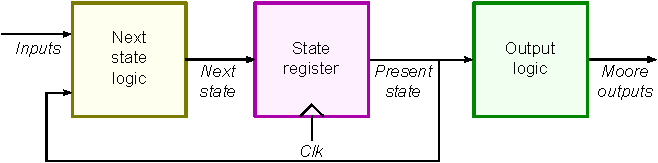
\includegraphics[width=.6\textwidth]{fsm_moore}\\[1mm]{\small Moore}\\[2mm]
  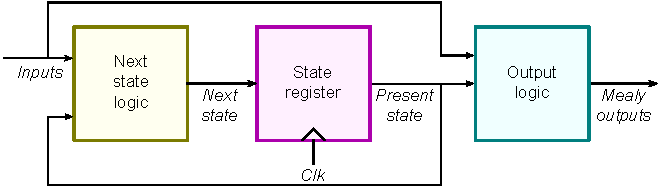
\includegraphics[width=.6\textwidth]{fsm_mealy}\\[1mm]{\small Mealy}
  \begin{columns}[t]
  \begin{column}{.48\textwidth}
    \begin{itemize}\scriptsize\itemsep2pt
      \item \alert{Moore}: output depends only on the \emph{state}. Inputs are sampled only at clock events: easy to analyse, but often needs more states.
    \end{itemize}
  \end{column}
  \begin{column}{.5\textwidth}
    \begin{itemize}\scriptsize\itemsep2pt
      \item \alert{Mealy}: output depends on state \emph{and input}, so it changes as soon as the input does: a cycle faster, fewer states, but possible glitches.
    \end{itemize}
  \end{column}
  \end{columns}
\end{frame}

\begin{frame}{State Machine Timing}
  \begin{columns}[c]
  \begin{column}{.45\textwidth}
    \centering
    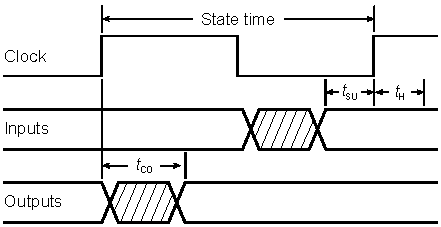
\includegraphics[width=\textwidth]{fsm_timing}
  \end{column}
  \begin{column}{.53\textwidth}
    \begin{itemize}\small\itemsep3pt
      \item The \alert{state time} is the interval between clocking events.
      \item At the edge, the present state and inputs are sampled; the next state and outputs are computed. New outputs are stable after $t_{CO}$.
      \item Inputs and next state must be stable for $t_{SU}$ before and $t_H$ after the edge. These set the FSM's maximum speed.
    \end{itemize}
  \end{column}
  \end{columns}
\end{frame}

\begin{frame}{State Diagrams}
  \begin{columns}[c]
  \begin{column}{.45\textwidth}
    \centering
    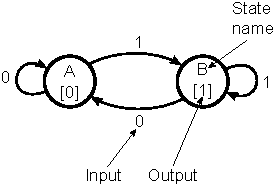
\includegraphics[width=.45\textwidth]{moore_template}\hspace{3mm}
    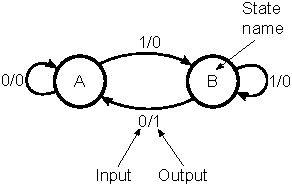
\includegraphics[width=.5\textwidth]{mealy_template}\\[1mm]
    {\small Moore \hspace{.2\textwidth} Mealy}
  \end{column}
  \begin{column}{.53\textwidth}
    \begin{itemize}\small\itemsep3pt
      \item \alert{States}: circles, one per state time.
      \item \alert{State names}: symbolic ($s_0$, \textit{idle}, \textit{ready}).
      \item \alert{Arrows}: transitions, labelled with input values; a state has an exit for every input combination: $2^n$ arrows for $n$ inputs. For larger $n$, arrows carry Boolean conditions (Chapter 15).
      \item \alert{Outputs}: Moore, inside the state; Mealy, after a ``/'' on the arrow.
    \end{itemize}
  \end{column}
  \end{columns}
\end{frame}

\begin{frame}{State Table}
  \begin{columns}[c]
  \begin{column}{.5\textwidth}
    \centering\small\striped
    \begin{tabular}{@{}cc|cc@{}}
      \toprule
      \makecell{Present\\state} & \makecell{Input\\$X$} & \makecell{Next\\state} & \makecell{Output\\$Y$} \\
      \midrule
      A & 0 & A & 0 \\ A & 1 & B & \\ B & 0 & A & 1 \\ B & 1 & B & \\
      \bottomrule
    \end{tabular}
  \end{column}
  \begin{column}{.48\textwidth}
    \begin{itemize}\small\itemsep3pt
      \item A truth table that includes the present state as an input and the next state as an output.
      \item Level-to-pulse converter, two states: in A with $X = 0$ stay in A; $X = 1$ go to B. In B, $X = 0$ returns to A; $X = 1$ stays in B.
    \end{itemize}
  \end{column}
  \end{columns}
\end{frame}

\begin{frame}{State Encoding}
  \begin{columns}[c]
  \begin{column}{.45\textwidth}
    \centering\scriptsize\striped
    \begin{tabular}{@{}cccc@{}}
      \toprule
      No & Binary & Gray & One-hot (8) \\
      \midrule
      0 & 000 & 000 & 00000001 \\ 1 & 001 & 001 & 00000010 \\ 2 & 010 & 011 & 00000100 \\ 3 & 011 & 010 & 00001000 \\
      4 & 100 & 110 & 00010000 \\ 5 & 101 & 111 & 00100000 \\ 6 & 110 & 101 & 01000000 \\ 7 & 111 & 100 & 10000000 \\
      \bottomrule
    \end{tabular}
  \end{column}
  \begin{column}{.53\textwidth}
    \begin{itemize}\scriptsize\itemsep3pt
      \item \alert{Binary}: $\lceil\log_2 N\rceil$ bits; fewest flip-flops, more decoding logic, several bits may change at once.
      \item \alert{Gray}: also $\lceil\log_2 N\rceil$ bits; successive codes differ in one bit; benefit depends on the transition order.
      \item \alert{Johnson}: $2k$ states from $k$ bits; one bit changes per step; more flip-flops.
      \item \alert{One-hot}: $N$ bits for $N$ states; simple decoding and often simpler logic, more flip-flops.
      \item Choose by states, speed, hardware and power.
    \end{itemize}
  \end{column}
  \end{columns}
\end{frame}

\begin{frame}{Example: Encoding 6 States}
  \centering\small\striped
  \begin{tabular}{@{}lcl@{}}
    \toprule
    \textbf{Encoding} & \textbf{Flip-flops} & \textbf{Note} \\
    \midrule
    Binary & $\lceil\log_2 6\rceil = 3$ & 2 unused patterns \\
    Gray & 3 & Successive codes differ by one bit \\
    Johnson & $\lceil 6/2\rceil = 3$ & $2k = 6$ states: 000, 001, 011, 111, 110, 100; no unused patterns \\
    One-hot & 6 & Each state is a single flip-flop \\
    \bottomrule
  \end{tabular}
  \begin{itemize}\small
    \item Binary, Gray and Johnson all need 3 flip-flops but are not interchangeable.
    \item One-hot uses twice as many flip-flops, but reading a state or an output is a direct read of one flip-flop.
  \end{itemize}
\end{frame}

%===============================================================================
\section{FSM Design}
%===============================================================================

\begin{frame}{The FSM Design Flow}
  \begin{columns}[c]
  \begin{column}{.5\textwidth}
    \centering
    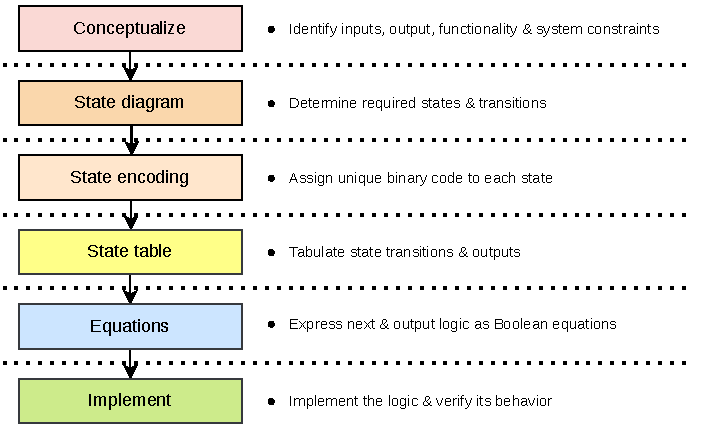
\includegraphics[width=\textwidth]{fsm_synthesis}
  \end{column}
  \begin{column}{.48\textwidth}
    \begin{itemize}\small\itemsep3pt
      \item Identify inputs, outputs and constraints; draw the \alert{state diagram}; \alert{encode} the states; build the \alert{state table}; derive next-state and output equations; implement and verify.
      \item Like combinational design, plus \alert{state assignment}.
      \item The first two steps need design judgement. When an FSM misbehaves, check the specification and state diagram first.
    \end{itemize}
  \end{column}
  \end{columns}
\end{frame}

%===============================================================================
\section{Level-to-Pulse Converter}
%===============================================================================

\begin{frame}{Level-to-Pulse Converter}
  \begin{columns}[c]
  \begin{column}{.5\textwidth}
    \centering
    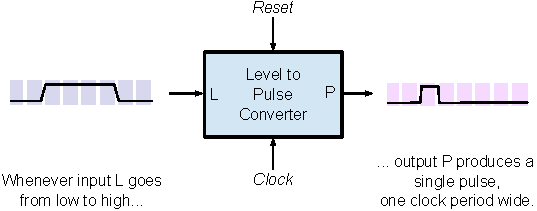
\includegraphics[width=.9\textwidth]{level2pulsetop}
  \end{column}
  \begin{column}{.48\textwidth}
    \begin{itemize}\small\itemsep3pt
      \item Outputs a \alert{single-cycle pulse} each time the input goes high, however long it stays high.
      \item An edge detector: a button press lasts many cycles, but a counter needs one clean enable.
    \end{itemize}
  \end{column}
  \end{columns}
  \centering
  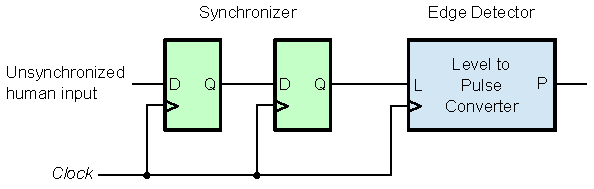
\includegraphics[width=.45\textwidth]{level2pulseblock}
  \begin{itemize}\small
    \item Human inputs are asynchronous: pass them through two series D flip-flops (a synchroniser), or the edge may fall inside setup/hold, the circuit captures an unpredictable value and fails.
  \end{itemize}
\end{frame}

\begin{frame}{Moore Version}
  \begin{columns}[c]
  \begin{column}{.5\textwidth}
    \centering
    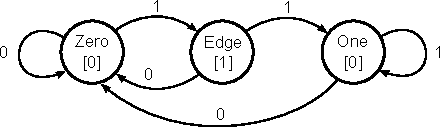
\includegraphics[width=\textwidth]{level2pulsestd}\\[2mm]
    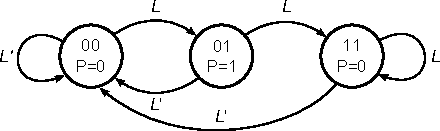
\includegraphics[width=\textwidth]{level2pulsestd2}
  \end{column}
  \begin{column}{.48\textwidth}
    \begin{itemize}\small\itemsep3pt
      \item Three states, encoded 00 (waiting), 01 (edge detected, $P = 1$), 11 (waiting for falling edge).
      \item The lower diagram spells out each transition condition: it scales to many inputs and outputs.
    \end{itemize}
  \end{column}
  \end{columns}
\end{frame}

\begin{frame}{Moore: State Table and Equations}
  \begin{columns}[c]
  \begin{column}{.48\textwidth}
    \centering\scriptsize\striped
    \begin{tabular}{@{}cc|c|cc|c@{}}
      \toprule
      $Q_1$ & $Q_0$ & $L$ & $Q_1^+$ & $Q_0^+$ & $P$ \\
      \midrule
      0&0&0&0&0&0 \\ 0&0&1&0&1&0 \\ 0&1&0&0&0&1 \\ 0&1&1&1&1&1 \\ 1&1&0&0&0&0 \\ 1&1&1&1&1&0 \\
      \bottomrule
    \end{tabular}\\[2mm]
    \small $Q_1^+ = LQ_0 \qquad Q_0^+ = L \qquad P = \overline{Q_1}Q_0$
  \end{column}
  \begin{column}{.5\textwidth}
    \centering
    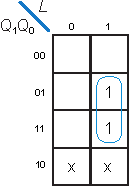
\includegraphics[height=.1\textheight]{level2pulsekmap1}\hspace{1mm}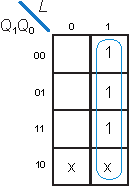
\includegraphics[height=.1\textheight]{level2pulsekmap2}\hspace{1mm}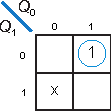
\includegraphics[height=.1\textheight]{level2pulsekmap3}\\[3mm]
    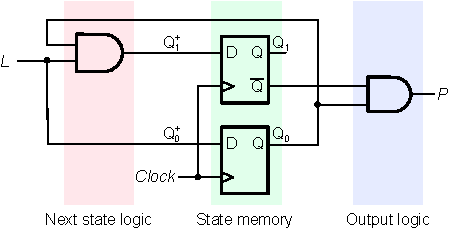
\includegraphics[width=.9\textwidth]{level2pulsesch}
  \end{column}
  \end{columns}
\end{frame}

\begin{frame}{Mealy Version: Two States}
  \begin{columns}[c]
  \begin{column}{.5\textwidth}
    \centering
    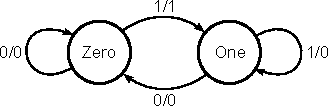
\includegraphics[width=.8\textwidth]{level2pulse3std}\\[2mm]
    \centering\small\striped
    \begin{tabular}{@{}c|c|c|c@{}}
      \toprule
      $Q$ & $L$ & $Q^+$ & $P$ \\
      \midrule
      0&0&0&0 \\ 0&1&1&1 \\ 1&0&0&0 \\ 1&1&1&0 \\
      \bottomrule
    \end{tabular}
  \end{column}
  \begin{column}{.48\textwidth}
    \begin{itemize}\small\itemsep3pt
      \item A Mealy output reacts to the input immediately, so no extra state is needed to hold the pulse.
      \item By inspection (no K-map): $Q^+ = L$, $P = \overline{Q}L$.
    \end{itemize}
    \centering
    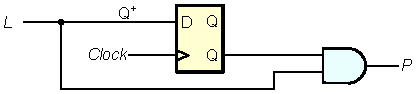
\includegraphics[width=.8\textwidth]{level2pulse2sch}
    \begin{itemize}\small
      \item One fewer state bit and flip-flop, simpler next-state logic.
    \end{itemize}
  \end{column}
  \end{columns}
\end{frame}

%===============================================================================
\section{Bit Sequence Detector}
%===============================================================================

\begin{frame}{Bit Sequence Detectors}
  \begin{enumerate}\small\itemsep4pt
    \item Define the sequence to detect; the output is active when it is fully recognised in the last state.
    \item Draw an initial state diagram for the \alert{ideal path}: the input is exactly the sequence from the start.
    \item Complete it: every state needs an exit for input 0 and one for input 1.
  \end{enumerate}
  \begin{block}{The 110 detector}
    \small Assert $z$ for one clock cycle whenever \texttt{110} appears, including overlapping occurrences.\\[1mm]
    \texttt{x: 1 1 0 0 0 1 1 0 1 1 1 1 0 0}\\
    \texttt{z: 0 0 1 0 0 0 0 1 0 0 0 0 1 0}
  \end{block}
\end{frame}

\begin{frame}{110 Detector: Moore Design}
  \begin{columns}[c]
  \begin{column}{.5\textwidth}
    \centering\small\striped
    \begin{tabular}{@{}cl@{}}
      \toprule
      State & Meaning \\
      \midrule
      $S_0$ & No matching bits \\ $S_1$ & First 1 found \\ $S_2$ & Second 1 found \\ $S_3$ & 0 found: assert $z$ \\
      \bottomrule
    \end{tabular}
    \begin{itemize}\small\itemsep3pt
      \item One state per bit of progress plus an idle state: four states.
    \end{itemize}
  \end{column}
  \begin{column}{.48\textwidth}
    \centering
    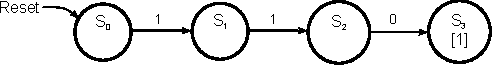
\includegraphics[width=.9\textwidth]{bsd1moore0_sd}\\[1mm]{\scriptsize Ideal path}\\[3mm]
    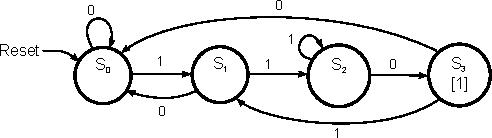
\includegraphics[width=.9\textwidth]{bsd1moore1_sd}\\[1mm]{\scriptsize Completed diagram}
  \end{column}
  \end{columns}
\end{frame}

\begin{frame}{Moore Detector: Table and Equations}
  \begin{columns}[c]
  \begin{column}{.45\textwidth}
    \centering\scriptsize\striped
    \begin{tabular}{@{}cc|c|cc|c@{}}
      \toprule
      $Q_1$ & $Q_0$ & $x$ & $Q_1^+$ & $Q_0^+$ & $z$ \\
      \midrule
      0&0&0&0&0&0 \\ 0&0&1&0&1&0 \\ 0&1&0&0&0&0 \\ 0&1&1&1&0&0 \\
      1&0&0&1&1&0 \\ 1&0&1&1&0&0 \\ 1&1&0&0&0&1 \\ 1&1&1&0&1&1 \\
      \bottomrule
    \end{tabular}\\[1mm]
    {\scriptsize $S_0 = 00,\ S_1 = 01,\ S_2 = 10,\ S_3 = 11$}
  \end{column}
  \begin{column}{.53\textwidth}
    \centering
    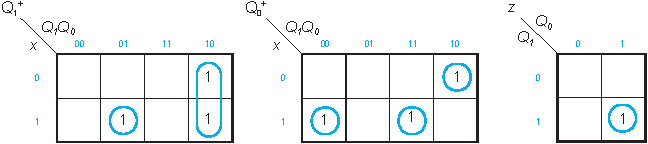
\includegraphics[width=.95\textwidth]{bsd1moore_kmap}
    \small
    \begin{align*}
      Q_1^+ &= Q_1\overline{Q_0} + \overline{Q_1}Q_0x \\
      Q_0^+ &= \overline{Q_1}\,\overline{Q_0}x + Q_1\overline{Q_0}\,\overline{x} + Q_1Q_0x \\
      z &= Q_1Q_0
    \end{align*}
  \end{column}
  \end{columns}
\end{frame}

\begin{frame}{Moore Detector: Schematic}
  \centering
  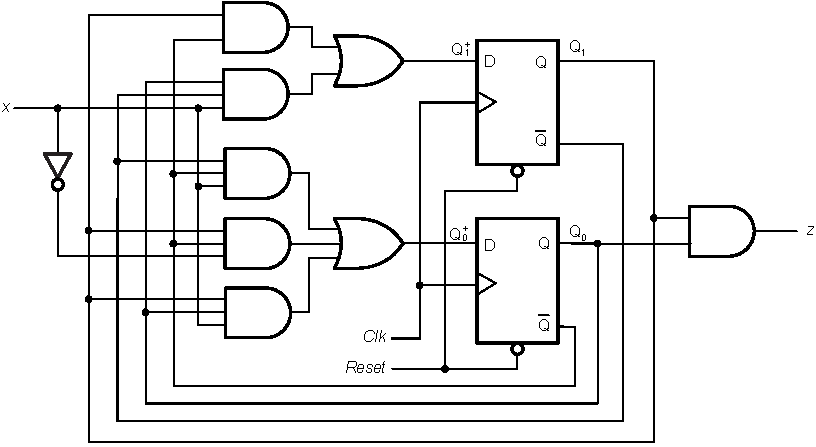
\includegraphics[height=.62\textheight]{bsdmoore_sch}
\end{frame}

\begin{frame}{110 Detector: Mealy Design}
  \begin{columns}[c]
  \begin{column}{.55\textwidth}
    \begin{itemize}\small\itemsep3pt
      \item Three states, not four: the output is asserted on the transition from $S_2$ back to $S_0$ (the 0 that completes \texttt{110}).
    \end{itemize}
    \centering
    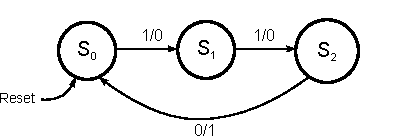
\includegraphics[width=.5\textwidth]{bsd1mealy_sd0}\hspace{2mm}
    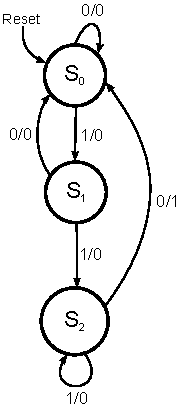
\includegraphics[height=.3\textheight]{bsd1mealy_sd}\\[1mm]
    {\scriptsize Ideal path \hspace{.15\textwidth} Completed}
  \end{column}
  \begin{column}{.43\textwidth}
    \centering\scriptsize\striped
    \begin{tabular}{@{}cc|c|cc|c@{}}
      \toprule
      $Q_1$ & $Q_0$ & $x$ & $Q_1^+$ & $Q_0^+$ & $z$ \\
      \midrule
      0&0&0&0&0&0 \\ 0&0&1&0&1&0 \\ 0&1&0&0&0&0 \\ 0&1&1&1&0&0 \\
      1&0&0&0&0&1 \\ 1&0&1&1&0&0 \\ 1&1&X&X&X&X \\
      \bottomrule
    \end{tabular}\\[1mm]
    {\scriptsize Code 11 is unused: don't cares.}
  \end{column}
  \end{columns}
\end{frame}

\begin{frame}{Mealy Detector: Equations}
  \centering
  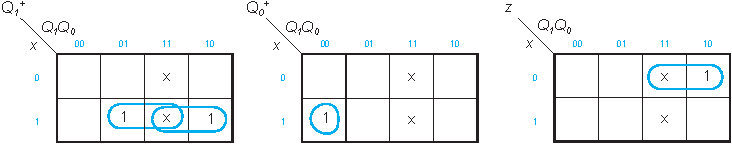
\includegraphics[width=.8\textwidth]{bsd1mealy_kmap}
  \begin{block}{Using the don't cares}
    \small $Q_1^+ = Q_1x + Q_0x \qquad Q_0^+ = \overline{Q_1}\,\overline{Q_0}x \qquad z = Q_1\overline{x}$
  \end{block}
  {\small Implementing the circuit is left as an exercise, following the Moore pattern.}
\end{frame}

%===============================================================================
\section{Practical Aspects}
%===============================================================================

\begin{frame}{Moore versus Mealy in Practice}
  \begin{columns}[c]
  \begin{column}{.45\textwidth}
    \centering
    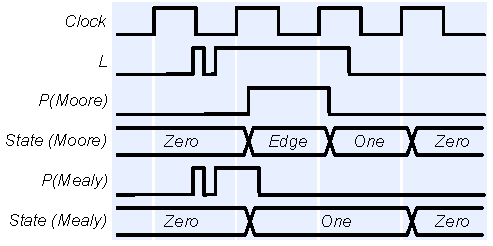
\includegraphics[width=\textwidth]{l2p_timing}
  \end{column}
  \begin{column}{.53\textwidth}
    \begin{itemize}\small\itemsep3pt
      \item Mealy: output $= f$(state, inputs). Moore: output $= f$(state).
      \item The input $L$ has a glitch between clock edges. The Moore machine looks only at values sampled at clock edges, so it ignores the glitch.
      \item The Mealy output follows $L$ between edges, so the glitch can reach the output. State transitions still use the value sampled at the edge.
    \end{itemize}
  \end{column}
  \end{columns}
\end{frame}

\begin{frame}{Registered (Synchronous) Mealy Outputs}
  \centering
  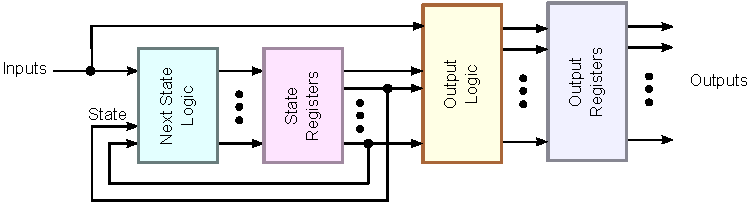
\includegraphics[width=.65\textwidth]{fsm_syncmealy}
  \begin{itemize}\small\itemsep3pt
    \item Moore outputs are easier to reason about. Mealy outputs respond faster and often need fewer states, but may glitch.
    \item Mealy outputs can upset other circuits or state machines they drive. Synchronous controls help but do not remove every timing concern.
    \item \alert{Registering} the outputs keeps them stable between clock edges, at the cost of one clock cycle of delay.
  \end{itemize}
\end{frame}

\begin{frame}{Back to the Opening Question}
  \begin{block}{The 110 detector}
    \small A plain counter walks a fixed sequence and cannot react to the data. An FSM can: one state per bit of progress ($S_0$ idle, $S_1$ one 1, $S_2$ two 1s), moving on a matching bit and falling back on a mismatch. In the Moore version a fourth state $S_3$ asserts $z$; in the Mealy version $z$ is asserted on the transition out of $S_2$ when $x = 0$.
  \end{block}
\end{frame}

%===============================================================================
\section{Summary}
%===============================================================================

\begin{frame}{Summary}
  \begin{itemize}\itemsep3pt\small
    \item A \alert{Moore} machine's output depends only on the current state: stable between clock edges.
    \item A \alert{Mealy} machine's output depends on state and input: it can respond within a cycle but may glitch.
    \item \alert{State encoding} (binary, Gray, one-hot) trades flip-flop count against logic complexity and speed.
    \item Design flow: state diagram $\to$ state table $\to$ state encoding $\to$ next-state and output equations $\to$ schematic.
    \item A state diagram is a specification of the machine's behaviour.
  \end{itemize}
  \begin{block}{Looking ahead}
    Chapter 14 reverses the direction: given a circuit, derive its state diagram. Chapter 15 extends design to controllers with several inputs and outputs.
  \end{block}
\end{frame}

\end{document}
